%%
%% pytorch-neural-doodle/docs/content/chapters/implementation.tex
%%
%% Created by Paul Warkentin <paul@warkentin.email> on 21/08/2018.
%% Updated by Bastian Boll <mail@bbboll.com> on 07/10/2018.
%%

\section{Implementation}
\label{section:implementation}

As a starting point, Champandard examines user behavior while authoring style transfers. This is made possible through a social media bot \cite{deepforger2015}, making artistic style transfer algorithms available to a general public. It can be observed, that in the cases where the algorithm does not meet the users expectation, it is often due to a lack of semantic segmentation of style and content images. As an example, when transfering an artists style to a photographic portrait, one would expect the algorithm to transfer the color and texture of skintones the artist chose to the skin areas of the portrait. While this expectation may at times be met, the patch based style loss constructed above does not generally enforce such a behavior. The usage of semantic segmentation is especially prominent in more specialized approaches to style transfer \cite{yang2017semantic}, suggesting additional merit to the presented intuition.

Note, that convolutional neural networks such as VGG do implicitly learn semantic segmentation of images \cite{thoma2016survey}, but this segmentation is not put to use in the above style loss construction because nearest neighbour patches are selected only with respect to similarity in texture. A segment of sky in the background of a style painting may absolutely be selected as nearest neighbour patch for a skintone area in the content picture, if local texture happens to be similar. This lack of semantic segmentation causes glitches and subverts the intention of the user but the disregard for the semantic segmentation extracted by the convolutional neural network is in some respects a byproduct of the design -- the style loss intentionally uses low layer responses to capture local texture information and to not capture higher level (content) responses such as semantic information. This leaves the user with a very limited number of control levers. Choosing the parameter \(\alpha\) which weights style loss against content loss presents a spectrum between a faithful reproduction of the content image and an unstructured reproduction of style texture with no regard to the content. This is insufficient in practice, especially for abstract styles and in those -- particularly interesting -- cases where style and content image are very dissimilar in perspective or subject.

The core idea of Champandard lies in incorporating segmentation from a semantic map both indirectly as part of the nearest neighbour patch computation and directly into the style loss term.

\subsection{Semantic maps}

A semantic map is an image dispaying a semantic segmentation of another image. It has the same aspect ratio as the segmented image and encodes semantically similar sections as areas with the same color. This information can be provided by a user as an artistic control lever of the process. In fact, as \cite{doodles2016} points out, it is possible to go one step further, encoding not only the semantic affilliation of pixels in a given area with each other, but also the relationship of different semantic areas. This is done, by choosing similar colors for the segmentation of semantically similar (but not equal) areas. When working with an image of a landscape, one may choose to segment different variations of woodland appearance with different shades of one color, say green.

The process of authoring semantic maps is technically easy, as will be described in the next section, but it can be artistically challenging. The latter can also be seen as opportunity: additional leeway in the artistic shaping of images presents the possibility of more appealing results. This fact has been noted by \cite{doodles2016} and is clearly corroborated through our experiments.

\subsection{Style Loss}

The semantic map of the style image is processed by the VGG network and activations for specific layers are gathered. In the case of a VGG 19 network, we choose the layers \texttt{conv3\_1} and \texttt{conv4\_1}. Denote the response tensor with \(m^s\). This tensor has two spatial dimensions and one channel dimension. The vector \(m^s\) is subsequently scaled by a factor \(\gamma\) and concatenated along the channel dimension with the response vector \(y^s\) of the style image
\[x^s = y \,||\,\gamma m \]
The analogous preparation steps are applied to the content image
\[x^c = y^c \,||\,\gamma m^c \]
For the reasons outlined in the introduction, a patch-based style loss approach is prefered over a Gram-based approach. We therefore compute \(k\times k\) patches \(\Psi (x^s)\) and \(\Psi (x^c)\) along the spatial dimensions. Our implementation specifically uses \(3\times 3\) patches. 

Given \(x^s\) and \(x^c\), the patch-based approach of \cite{mrf2016} can be applied without the need for significant changes. Nearest neighbour patches are computed with respect to normalized cross-correlation and we have the finished patch-based style loss
\[\mathcal{L}_{s,p}(x^s,x^c) = \sum_i \|\Psi_i(x^c)-\Psi_{\text{NN}(i)}(x^s)\|_2^2\]

The parameter \(\gamma\) can be seen as a user control point, specifying how heavily the segmentation should be weighted against local pixel conformance during nearest neighbour computation. This specific way of incorporating segmentation maps has two principal upsides:
\begin{enumerate}
	\item The segmentation maps can easily be authored, as they do not need to conform to many formal specifications. They can have an arbitrary number of channels and can be drawn with a reduced resolution as compared to the original style- and content image. These are both conveniences in practical use.
	% embedding segmentation
	\item The algorithm being used is essentially the same as the patch based approach of \cite{mrf2016} because the datastructure being worked on does only change along the channel dimension and the operations being applied remain the same. In the common library implementation of respective convolutions, one does not need to change anything. The only extra implementation is the weighted concatenation of segmentation maps.
\end{enumerate}

Manual work can be saved by using a lower resolution for the segmentations and computational effort as well as memory can be saved by increasing the stride between successive patches. Neither of these simplifications have a large impact on practical results.

\subsection{Content Loss}

Content loss can be added without additional modifications to the original approach of Gatys et al. \cite{gatys2015neural}. With regard to semantic maps, it merits mentioning that much like the original implementation of \cite{doodles2016}, our present implementation can be run in a mode that requires a content segmentation but does not require a content image. In this mode, texture is merely semantically transfered from the style image to the content image. Content loss ist omitted, the total loss being minimized is exactly the style loss. Figure \ref{fig::nocontent} shows results for this mode. This is what the title of the present work refers to as a \textbf{Neural Doodle}.

\begin{figure}
	\begin{subfigure}[t]{0.32\textwidth}
		\centering
		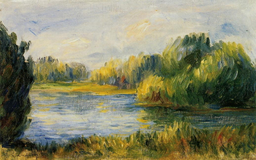
\includegraphics[width=4.5cm]{renoir/renoir.png}
	\end{subfigure}%\hspace{5mm}
	~
	\begin{subfigure}[t]{0.32\textwidth}
		\centering
		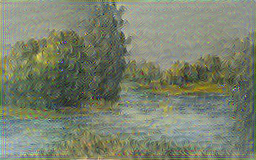
\includegraphics[width=4.5cm]{renoir/out_result.png}
	\end{subfigure}%\hspace{5mm}
	~
	\begin{subfigure}[t]{0.32\textwidth}
		\centering
		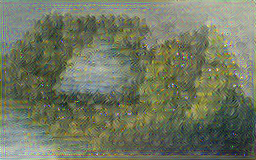
\includegraphics[width=4.5cm]{renoir/out2_result.png}
	\end{subfigure}
	\\
	\begin{subfigure}[t]{0.32\textwidth}
		\centering
		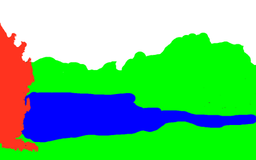
\includegraphics[width=4.5cm]{renoir/renoir_style.png}
	\end{subfigure}%\hspace{5mm}
	~
	\begin{subfigure}[t]{0.32\textwidth}
		\centering
		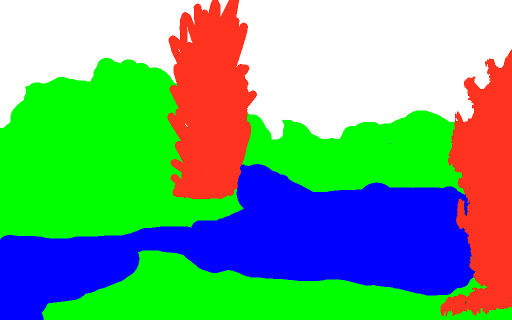
\includegraphics[width=4.5cm]{renoir/renoir_out_style.png}
	\end{subfigure}%\hspace{5mm}
	~
	\begin{subfigure}[t]{0.32\textwidth}
		\centering
		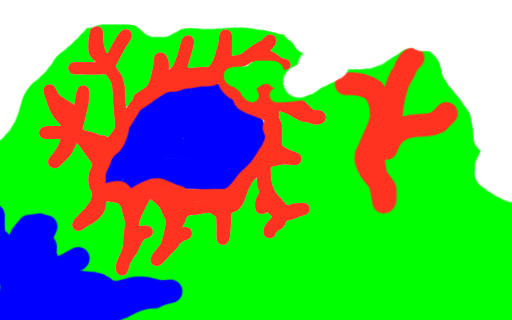
\includegraphics[width=4.5cm]{renoir/renoir_out_style_2.png}
	\end{subfigure}
	\caption[]{Reproduction of the paper results generated by our implementation. Original style image (Renoir) with respective segmentation in the left column. Two different segmentation maps (lower row) and respective transfer results (upper row). No content image was used and the content loss omitted.}
	\label{fig::nocontent}
\end{figure}
